\begin{figure*}
  \centering
    \centerline{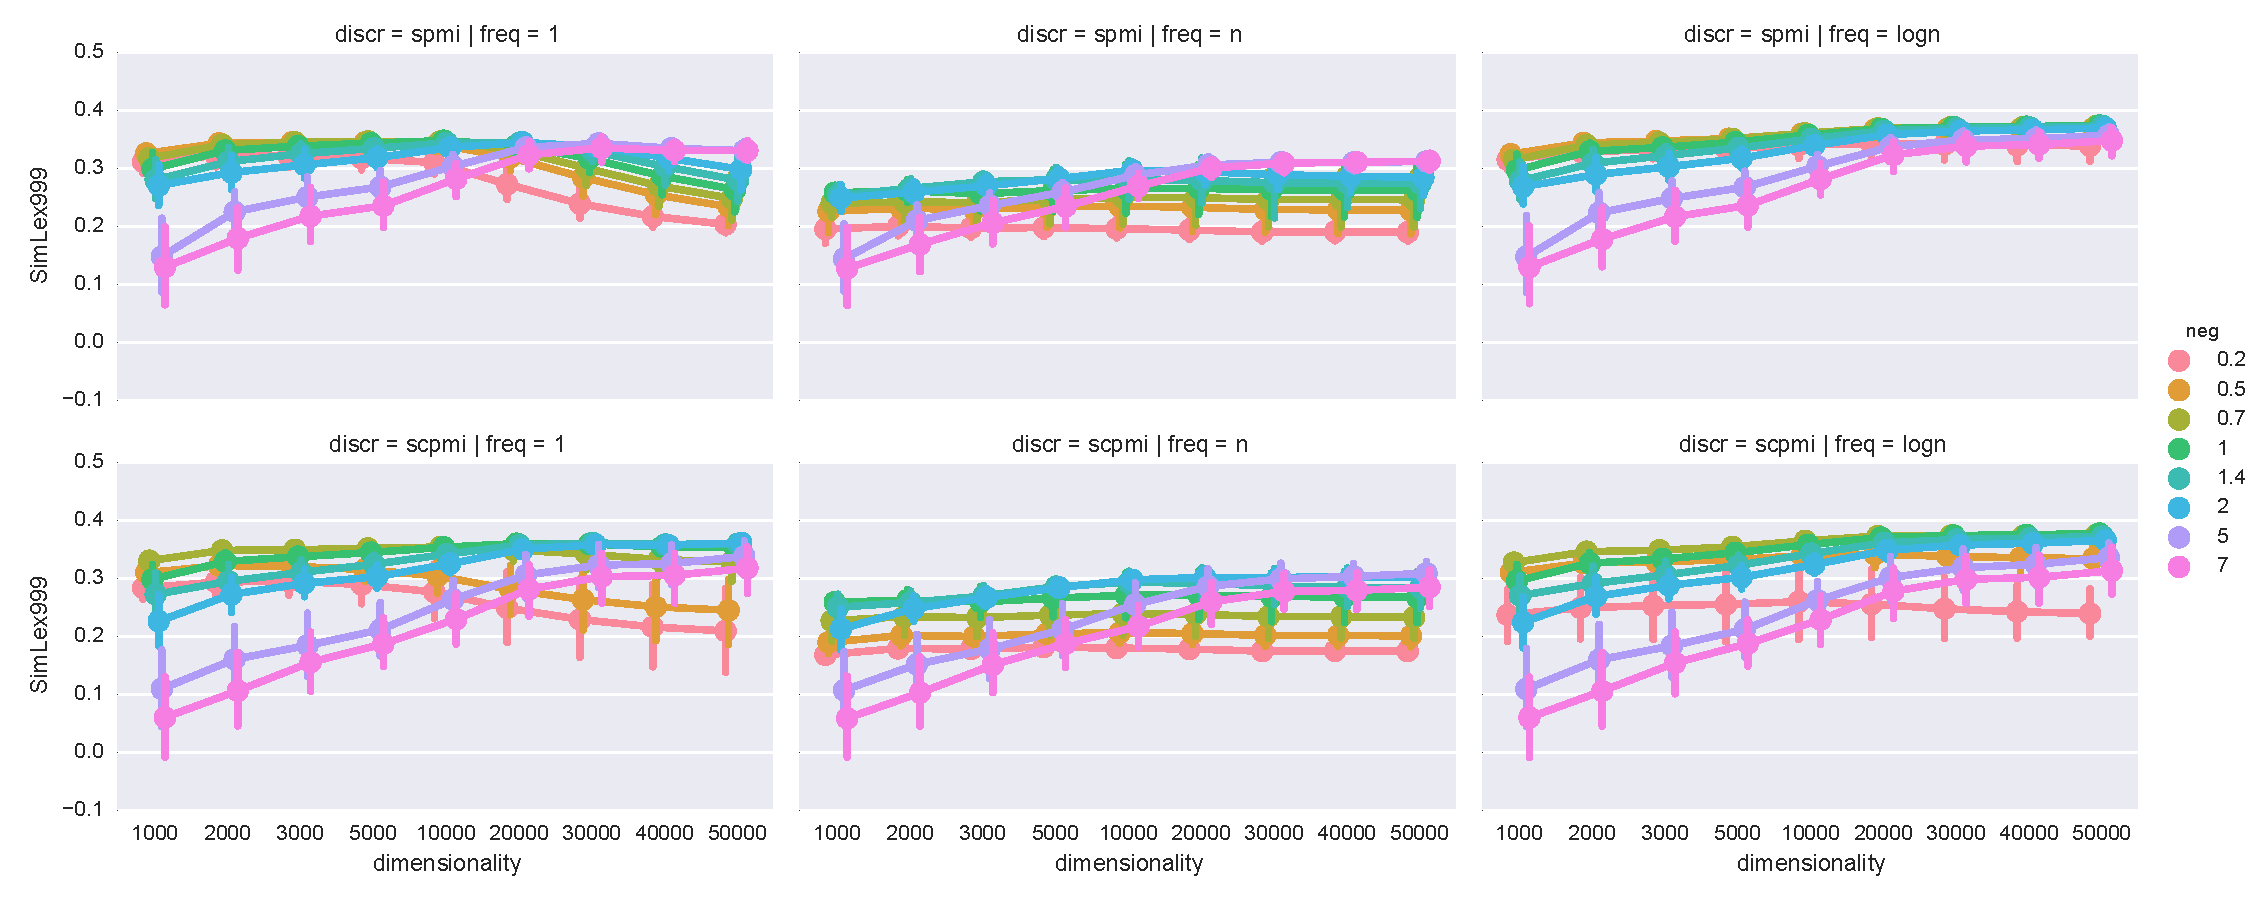
\includegraphics[width=1.11\textwidth]{supplement/figures/SimLex999-interaction-neg}}
    \caption{\textbf{The behaviour of shifted PMI (SPMI) on SimLex-999.} \texttt{discr=spmi}, \texttt{freq=1} and \texttt{neg=1} corresponds to positive PMI. Error bars correspond to a 95\% confidence interval as the value is estimated by averaging over all the values of the omitted parameters: \texttt{cds} and similarity.}
    \label{fig:interaction-neg}
\end{figure*}

%%% Local Variables:
%%% mode: latex
%%% TeX-master: "paper"
%%% End:
